\documentclass[11pt]{article}
\usepackage[T1]{fontenc}
\usepackage[utf8]{inputenc}
\usepackage{lmodern}
\usepackage[margin=1in]{geometry}
\usepackage{microtype}
\usepackage{amsmath,amssymb,amsthm,mathtools}
\usepackage{booktabs,longtable,array}
\usepackage{enumitem}
\usepackage{xcolor}
\usepackage{hyperref}
\usepackage{listings}
\usepackage{tikz}
\usetikzlibrary{arrows.meta,positioning,fit}

\hypersetup{colorlinks=true,linkcolor=blue!45!black,citecolor=blue!45!black,urlcolor=blue!45!black}
\lstset{basicstyle=\ttfamily\small,breaklines=true,frame=single,columns=fullflexible,keepspaces=true}
\setlist[itemize]{topsep=3pt,itemsep=2pt,parsep=1pt}
\setlist[enumerate]{topsep=3pt,itemsep=2pt,parsep=1pt}

\newcommand{\MeTTa}{\textup{MeTTa}}
\newcommand{\MeTTaIL}{\textup{MeTTaIL}}
\newcommand{\Megalodon}{\textup{Megalodon}}
\newcommand{\HOTG}{\textup{HOTG}}
\newcommand{\DTT}{\textup{DTT}}
\newcommand{\MTT}{\textup{MTT}}
\newcommand{\MATT}{\textup{MATT}}
\newcommand{\OSLF}{\textup{OSLF}}
\newcommand{\Lean}{\textup{Lean}}
\newcommand{\Coq}{\textup{Coq}}
\newcommand{\Agda}{\textup{Agda}}
\newcommand{\PureKernel}{\textup{PureKernel}}
\newcommand{\PureMeTTa}{\textup{PureMeTTa}}
\newcommand{\MMT}{\textup{MMT}}
\newcommand{\code}[1]{\texttt{#1}}
\newcommand{\Fact}{\textbf{Grounded fact.}}
\newcommand{\Infer}{\textbf{Design inference.}}
\newcommand{\Open}{\textbf{Open obligation.}}

\title{A Grounded Design Memo for a Self-Covering \MeTTa{} Proof Kernel\\
\large HOTG, dependent type theory, Megalodon, MeTTa-Pure, MeTTaIL, OSLF, and MTT/MATT}
\author{Prepared for Zar by Oru\v{z}i}
\date{June 2026}

\begin{document}
\maketitle

\begin{abstract}
This memo restates only the grounded, useful content from the discussion about a \MeTTa{} proof kernel capable of supporting both \HOTG{}-style classical higher-order set theory and constructive/dependent type theory.  It deliberately separates facts verified from source repositories and papers from design inferences and open hypotheses.  The core correction is that \Megalodon{} is not merely an ``external oracle'': its repository shows a compact proof checker with proof terms, lambdas, a simple type language, conversion, theorem/proof documents, hash-addressed imports, and multiple object theories.  That changes the design center.  The right target is a small \MeTTa{} trusted waist that can host multiple proof calculi and theory presentations, while keeping runtime execution, optimization, and general \MeTTa{} rewriting outside the unchecked logical core unless they enter through checked specifications or certificates.
\end{abstract}

\tableofcontents

\section{Status and epistemic hygiene}

This document is not a final foundation for \MeTTa{}.  It is a grounded design memo.
The earlier file \code{dtt\_hotg\_metta\_brainstorming\_cum\_heartstorming} is explicitly a brainstorming and heart-storming document, not final project knowledge.  It contains useful ideas, wrong turns, and model-generated speculation.  Therefore this memo uses three labels.

\begin{description}
\item[Grounded fact.] Something observed directly in the \Megalodon{}, \MeTTaIL{}, \OSLF{}, or \PureMeTTa{} sources, or in a cited paper/manual.
\item[Design inference.] A conclusion that follows reasonably from the facts and project goals, but still requires implementation and proof.
\item[Open obligation.] A theorem, engineering proof, benchmark, or artifact that must exist before the inference becomes trusted.
\end{description}

The guiding correction is simple: covering or embedding \Lean{}, \Megalodon{}, Isabelle/Pure, \DTT{}, \HOTG{}, or \MATT{} is not the same thing as outsourcing trust to external oracles.  The ideal is self-covering: faithful internal models, checked translations, and commutative coherence diagrams that make our own system more correct.

\section{What the \Megalodon{} repository actually shows}

\subsection{Megalodon is a proof checker with multiple theories}

\Fact{} The repository README says \Megalodon{} is ``an open source interactive theorem prover and proof checker'' whose main application is Proofgold documents.  It supports four Proofgold theories: Egal \HOTG{}, Mizar \HOTG{}, hereditarily finite sets, and an intuitionistic HOAS theory.  Egal is the default theory.  This is not hearsay; it is in the repository README.\cite{megalodon-readme}

\Fact{} The installation notes show command-line support for theory selection and proof/document infrastructure: \code{-hf}, \code{-hoas}, \code{-mizar}, \code{-I} for signature files, \code{-owned} for ownership files, and \code{-pfg} for Proofgold output.  Signature files are explicitly not allowed to contain proofs.\cite{megalodon-install}

\Infer{} \Megalodon{} is best read as evidence for a small kernel/framework design: one compact checking core, several theories above it, and a web-of-trust/import layer.  It should not be dismissed as a mere classical-set-theory oracle.  It is a useful proof-kernel exemplar and a covering target.

\subsection{The core proof calculus is small and lambda/proof-term based}

\Fact{} \Megalodon{}'s exported syntax interface contains a tiny type language:
\[
\code{TpVar},\quad \code{Prop},\quad \code{Set},\quad \code{Ar(tp,tp)}.
\]
Terms include de Bruijn variables, global term hashes, primitives, type application, term application, lambda, implication, and universal quantification.  Proofs include hypotheses, known theorem hashes, type application, term application, proof application, proof lambda, and type lambda.\cite{megalodon-syntax}

In abbreviated form, the interface is:

\begin{lstlisting}[caption={Megalodon core syntax shape, abbreviated from src/syntax.mli}]
type tp = TpVar of int | Prop | Set | Ar of tp * tp

type tm =
  | DB of int | TmH of string | Prim of int
  | TpAp of tm * tp | Ap of tm * tm | Lam of tp * tm
  | Imp of tm * tm | All of tp * tm

type pf =
  | Hyp of int | Known of string
  | PTpAp of pf * tp | PTmAp of pf * tm | PPfAp of pf * pf
  | PLam of tm * pf | TLam of tp * pf
\end{lstlisting}

\Fact{} The checker extracts and checks term types; application requires a function type, lambda forms an arrow type, implication and universal quantification are checked as propositions.  The proof checker handles universal instantiation, implication elimination, proof lambda, and type lambda.  Proposition checking reduces to conversion between the extracted proposition and the expected proposition.\cite{megalodon-termcheck,megalodon-proofcheck}

\Fact{} Conversion is based on beta/eta normalization plus controlled delta expansion of definitions.  It is not arbitrary \MeTTa{} rewriting.\cite{megalodon-conv}

\Infer{} \Megalodon{}'s ``C-like'' strength comes from a very small, permissive logical kernel plus powerful object theories, libraries, imports, and automation.  This supports Zar's intuition that a \MeTTa{} proof kernel should be made purer by separating the framework from theory-specific commitments.  It does \emph{not} imply that the exact \Megalodon{} calculus is sufficient for native dependent type theory.

\subsection{Megalodon has a visible web-of-trust layer}

\Fact{} The examples README explains that previous definitions may be referred to opaquely by Merkle roots or transparently by definitions.  The \code{-owned} option supplies an ownership file listing definitions and theorems published in Proofgold.  Megalodon warns if an axiom has not yet been proven and errors if a definition hash is not listed in the ownership file.\cite{megalodon-examples}

\Fact{} The same examples README mentions a translation of Metamath's \code{set.mm} into 40,558 \Megalodon{}-checkable theorems and an older Mizar Mathematical Library snapshot in \Megalodon{} format, though without proofs.\cite{megalodon-examples}

\Infer{} For \MeTTa{}, imports should be explicit proof-provenance objects: name, content hash, theory, axioms used, checker profile, dependencies, and trust status.  \Megalodon{} and Proofgold make that reality visible rather than pretending import trust is invisible.

\subsection{The user's 4CT project is a concrete Megalodon proof artifact}

\Fact{} The \code{zariuq/ai-agents} \code{megalodon/4CT} README states that it contains kernel-verified Megalodon proofs with exit code 0 refuting a specific Goertzel 4CT proof approach.  It lists verified files and commands to run Megalodon over them.\cite{zariuq-4ct-readme}

\Fact{} The file \code{lemma43\_refutation.mg} shows ordinary Megalodon proof structure: \code{Variable}, \code{Hypothesis}, \code{Definition}, \code{Theorem}, \code{let}, \code{assume}, \code{prove}, \code{apply}, \code{exact}, and \code{Qed}.\cite{zariuq-4ct-lemma}

\Infer{} This is useful because it shows \HOTG{}/set-style proof checking is not an abstract preference.  It is already being used in the project to catch real mathematical errors.  A future \MeTTa{} kernel should learn from this proof style, import style, and minimal checker discipline.

\section{What the existing \MeTTa{} artifacts already show}

\subsection{PureMeTTa already points to one surface, one core, two honest targets}

\Fact{} \code{PureMeTTa.tex} says the central claim is that the project should converge to a single elaborated \MeTTa-Core compiling to two honest targets: a trusted proof-oriented \MeTTa-Pure/PureKernel target and an efficient runtime execution seam backed by MORK/MM2 RuntimeExec.\cite{puremetta}

\Fact{} The same document compares this to the \Lean{}-style pattern:
\[
\text{surface language} \to \text{elaborated core} \to \text{checked kernel and compiled runtime}.
\]
It also emphasizes a closed proof-side semantic waist with canonical normalization, bidirectional checking, parser-free checked canonical evaluation, and preservation.\cite{puremetta}

\Fact{} The current proof-side branch is described as \MeTTa-Pure \(\to\) PureKernel \(\to\) A \(\to\) B \(\to\) C1, with theorem-level bridge files and a live trusted path through theoremic checking and canonicalization rather than a front-door evaluator.\cite{puremetta-proof}

\Infer{} The current \MeTTa-Pure direction is already close to the right shape: proof kernel and runtime are connected but not confused.  The next refinement is to make the proof kernel more theory-parametric, so that \HOTG{}-like and \DTT{}-like systems can both be covered without hardcoding either one as the only foundation.

\subsection{MeTTaIL and OSLF already connect operational descriptions to type/modal structure}

\Fact{} \code{MeTTaIL.tex} describes \MeTTaIL{} as a Lean 4 framework for pattern-matching rewrite rules with typed premises, a declarative one-step semantics, a proved sound-and-complete executable engine, and automatic derivation of an \OSLF{} behavioral type system for each \code{LanguageDef}.\cite{mettail}

\Fact{} \code{TypeSynthesis.lean} states the pipeline explicitly:
\[
\code{LanguageDef} \to \code{RewriteSystem} \to \code{ReductionSpan} \to \code{OSLFTypeSystem},
\]
with predicates, \(\Diamond\), \(\Box\), and a Galois connection.  It says the Galois connection \(\Diamond \dashv \Box\) follows automatically from a generic theorem.\cite{oslf-typesynthesis}

\Fact{} The same code defines an executable reduction relation and a declarative reduction relation, and proves the equivalence theorem \code{langReducesUsing\_iff\_execUsing}.\cite{oslf-typesynthesis}

\Fact{} \code{TypeSynthesis.lean} defines \code{langDiamondUsing}, \code{langBoxUsing}, \code{langGaloisUsing}, and \code{langOSLFUsing}; it then packages a generated \code{OSLFTypeSystem}.\cite{oslf-typesynthesis2}

\Infer{} \MeTTaIL{} is not just a compiler-compiler toy.  It is close to a theory/specification language for operational calculi.  However, a \MeTTaIL{} rewrite rule is not automatically a kernel conversion rule.  Rules must be classified.

\begin{center}
\begin{tabular}{@{}lll@{}}
\toprule
Rule class & Logical role & Kernel status \\
\midrule
Definitional reduction & Conversion/equality checking & trusted only if terminating/confluent/admitted \\
Operational step & Runtime/EvalSpec transition & reasoned about propositionally/modal-logically \\
Optimization rewrite & Compiler/runtime specialization & accepted by certificate/proof \\
Grounded oracle & FFI/host behavior & admitted only via biform contract \\
\bottomrule
\end{tabular}
\end{center}

\Infer{} Implementing \OSLF{}-like synthesis inside \MeTTa{}/CeTTa can be highly valuable, especially as a precompilation and specialization layer.  It should not automatically enlarge the trusted conversion kernel.  It should generate obligations, derived types, modalities, and certificates that the kernel can check.

\section{What Lean, Isabelle/Pure, Dedukti, MMT, MTT, and MATT contribute}

\subsection{Lean is not merely trace verification}

\Fact{} \Lean{}'s reference manual says Lean is based on the Calculus of Inductive Constructions with dependent functions, inductive types, a universe hierarchy, and impredicative proof-irrelevant \code{Prop}.  The pure fragment has a computational interpretation with canonical normal forms.  Classical axioms such as propositional extensionality, quotient principles, and choice are compatible with code generation partly because proofs and types can be erased, but they can block kernel computation.\cite{lean-axioms}

\Infer{} Lean's kernel checking is not merely trace verification.  Tactics and automation generate elaborated terms which the kernel checks in a global environment.  Trace/certificate checking is one possible proof-producing pattern, but Lean's main trust story is small-kernel checking of elaborated terms, plus separate compilation/extraction mechanisms.  For \MeTTa{}, the ideal is both:
\begin{enumerate}
\item ahead-of-time verification of the abstract machine, compiler, and runtime semantics where possible;
\item post-run trace/certificate checking for concrete executions and optimizations.
\end{enumerate}

\subsection{Isabelle/Pure, Dedukti, and MMT are framework exemplars}

\Fact{} Isabelle/Pure is the classic example of a generic theorem-prover meta-logic: rules are represented as propositions and proofs are built by combining rules; object logics are formalized in the meta-logic.\cite{isabelle-pure}

\Fact{} Dedukti's \(\lambda\Pi\)-calculus modulo theory is a logical framework capable of representing many theories, including constructive and classical predicate logic, simple type theory, pure type systems, CIC-like universes, and libraries translated from other systems.\cite{dedukti}

\Fact{} MMT is a theory/morphism framework in which logics, logical frameworks, and foundations can be represented as theories.  It is a benchmark for foundation-independent organization.\cite{mmt}

\Infer{} The \MeTTa{} kernel should not blindly copy Dedukti, Isabelle, MMT, Lean, or Megalodon.  They are benchmarks.  The question is:
\begin{quote}
What is the smallest \MeTTa{} waist that supports proof terms, theory specifications, object theories, reductions, imports, mode/morphism structure, runtime certificates, and coherent translations?
\end{quote}

\subsection{MTT and MATT are mode-theoretic organizers, not magic strength engines}

\Fact{} Multimodal Dependent Type Theory is parameterized by a mode theory containing modes, modalities, and transformations.  Its examples include guarded recursion, cohesion, and parametric quantification.\cite{mtt}

\Fact{} Shulman's multimodal adjoint type theory adds adjoint positive/negative modalities and gives semantics in diagrams of toposes and geometric morphisms.  This provides an architectural language for modes connected by adjoints.\cite{matt}

\Infer{} \MTT{}/\MATT{} is not primarily how one gets \HOTG{}'s large set-theoretic strength.  Strength comes from axioms, universes, and object theories.  \MTT{}/\MATT{} is how one organizes different worlds: proof, program, runtime trace, classical set semantics, constructive computation, capabilities, resources, staging, and evidence state.

\section{Does Megalodon change the design? Yes.}

The added Megalodon information changes the design center in four ways.

\paragraph{First.} The target should not be framed as ``DTT kernel plus external HOTG oracle.''  \Megalodon{} itself is a compact proof-term/kernel system with multiple theories.  A \MeTTa{} proof kernel can aspire to cover this style internally.

\paragraph{Second.} \HOTG{} support is not merely a semantic add-on.  It may be one of the cleanest ways to reason about ordinary extensional mathematics, set-like MeTTa semantics, nondeterministic execution relations, large corpora, and classical automation.

\paragraph{Third.} The proof kernel should become more parametric and therefore more pure.  If \HOTG{} and \DTT{} both have to fit, then the kernel is pressured away from ad hoc Lean imitation and away from ad hoc set-theory primitives.  The common waist becomes smaller: binding, terms, proofs, declarations, conversion, imports, theory specifications, and certificates.

\paragraph{Fourth.} The hard part shifts from ``which one foundation wins?'' to ``which parts are kernel-common, which are object-theory-specific, and which are mode/morphism structure?''

\section{Proposed kernel architecture}

Let \(\Sigma\) be the elaborated \MeTTa{} artifact waist.  It is not the entire runtime and not one monolithic logic.  It is the checked representation where proofs, programs, theories, imports, and certificates can meet.

\begin{center}
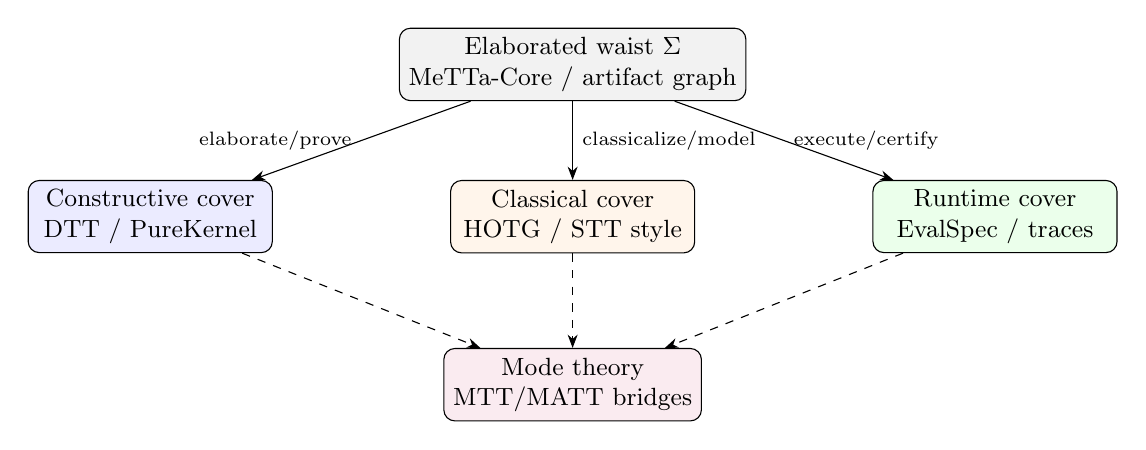
\begin{tikzpicture}[node distance=1.0cm and 1.6cm]
  \tikzset{box/.style={draw,rounded corners,align=center,minimum width=3.1cm,minimum height=.75cm,font=\small}}
  \node[box,fill=gray!10] (sigma) {Elaborated waist $\Sigma$\\MeTTa-Core / artifact graph};
  \node[box,fill=blue!8,below left=of sigma] (dtt) {Constructive cover\\DTT / PureKernel};
  \node[box,fill=orange!8,below=of sigma] (hotg) {Classical cover\\HOTG / STT style};
  \node[box,fill=green!8,below right=of sigma] (rt) {Runtime cover\\EvalSpec / traces};
  \node[box,fill=purple!8,below=1.2cm of hotg] (matt) {Mode theory\\MTT/MATT bridges};
  \draw[-{Stealth}] (sigma) -- node[left,font=\scriptsize]{elaborate/prove} (dtt);
  \draw[-{Stealth}] (sigma) -- node[right,font=\scriptsize]{classicalize/model} (hotg);
  \draw[-{Stealth}] (sigma) -- node[right,font=\scriptsize]{execute/certify} (rt);
  \draw[-{Stealth},dashed] (dtt) -- (matt);
  \draw[-{Stealth},dashed] (hotg) -- (matt);
  \draw[-{Stealth},dashed] (rt) -- (matt);
\end{tikzpicture}
\end{center}

The trusted kernel should be decomposed into these components.

\subsection{Framework core}

The framework core should provide:

\begin{enumerate}
\item names, de Bruijn or locally nameless binding, alpha-safe substitution, and hashing/content identity;
\item a small type/proposition/proof object language sufficient to express object-theory rules;
\item declarations: parameters, definitions, axioms, theorems, inductive/recursor declarations, and imports;
\item conversion: beta/eta plus admitted definitional reductions, always under a decidability discipline;
\item a proof checker for hypotheses, known theorems, instantiation, implication/application, abstraction, and theory-specific rules;
\item provenance: axioms used, imports used, hashes used, checker version, conversion profile, and trust level.
\end{enumerate}

\subsection{Object theory layer}

Above the framework core sit theory packages:

\begin{description}
\item[HOTG/STT profile.] Simple types with \code{Prop}, \code{Set}, arrows, universal quantification, implication, equality, membership, set constructors, choice/epsilon, and Tarski-Grothendieck axioms.  Megalodon's \code{tp}, \code{tm}, and \code{pf} syntax is a concrete reference point.
\item[DTT profile.] Dependent contexts, \(\Pi\), \(\Sigma\), universes, identity/equality, inductives, recursors, iota rules, universe constraints, and a decidable conversion relation for the proof-bearing fragment.
\item[HoTT/cubical profile, optional.] Path/equivalence structure, univalence, higher inductives, cubical computation if supported.  This is a later profile, not an assumption for the first kernel.
\item[Runtime/EvalSpec profile.] Operational semantics of \MeTTa{} programs as relations/traces, not as unconstrained definitional equality.
\item[Modal/mode profile.] Modes, modalities, transformations, adjunctions, resource/capability/staging worlds, and bridges between proof/runtime/classical/set worlds.
\end{description}

\subsection{Conversion discipline}

Conversion is the danger line.  For both \HOTG{} and \DTT{} support, conversion should be:

\begin{enumerate}
\item decidable in the proof-bearing fragment;
\item small enough to audit;
\item parameterized by a theory profile;
\item closed under checked declarations only;
\item never equal to full \MeTTa{} runtime rewriting unless that fragment is separately proved terminating, confluent, and sound for definitional equality.
\end{enumerate}

\subsection{Imports and web of trust}

The \Megalodon{}/Proofgold pattern suggests an explicit import object:

\begin{lstlisting}[caption={Sketch: proof provenance object}]
ProofArtifact := {
  theory          : TheoryId,
  statement       : TermHash,
  proof           : ProofHash,
  checkerProfile  : KernelProfileHash,
  conversion      : ConversionProfileHash,
  imports         : List ImportHash,
  axiomsUsed      : List AxiomHash,
  status          : proved | assumed | imported | stale | rejected,
  source          : local | chain | generated | external
}
\end{lstlisting}

\Infer{} Lean-like module imports, Megalodon/Proofgold-style hash imports, MMT-style theory morphisms, and \MeTTa{} atomspace objects should converge here.  This would make trust explicit and queryable.

\section{What modifications are needed to make MeTTa-Pure support both HOTG and DTT?}

\subsection{Modification 1: make theories first-class}

\MeTTa-Pure should not merely have a hardcoded DTT kernel plus ad hoc classical axioms.  It should have first-class theory descriptors:

\begin{lstlisting}[caption={Sketch: theory descriptor}]
Theory := {
  sorts       : SortSpec,
  terms       : TermConstructors,
  proofs      : ProofConstructors,
  constants   : ConstantDeclarations,
  reductions  : DefinitionalReductionRules,
  axioms      : AxiomDeclarations,
  inductives  : InductiveDeclarations,
  imports     : ImportDeclarations,
  modes       : Optional ModeSignature
}
\end{lstlisting}

For \HOTG{}, this descriptor can look \Megalodon{}-like.  For \DTT{}, it must include dependent binders, universe levels, inductive families, and recursor computation.

\subsection{Modification 2: add a simple-type/HOTG profile}

A \HOTG{} profile should include something close to Megalodon's minimal type grammar:
\[
A ::= \alpha \mid \code{Prop} \mid \code{Set} \mid A \to B.
\]
Terms need lambda/application, forall/implication propositions, equality, membership, primitive set constructors, and TG axioms.  The object theory can be classical and extensional.  Its proof checker can remain small.

This profile should not be optimized for numeric computation.  Church numerals and set encodings may be acceptable for proof-checking classical mathematics, but they are not ideal for runtime execution.  That is a library/tactic/compiler issue for HOTG, not a reason to pollute the core kernel.

\subsection{Modification 3: add a dependent profile}

A constructive/dependent profile needs:

\begin{enumerate}
\item contexts \(\Gamma\) with dependent declarations;
\item \(\Pi\)-types and lambdas with dependent substitution;
\item \(\Sigma\)-types and pairs/projections;
\item universes \(\mathcal{U}_0,\mathcal{U}_1,\ldots\), with clear predicativity/cumulativity rules;
\item identity/equality types;
\item inductive declarations with generated recursors/eliminators;
\item iota computation rules generated from declarations, not hand-coded per family;
\item subject reduction, decidable conversion, and universe consistency obligations.
\end{enumerate}

\subsection{Modification 4: classify MeTTaIL rewrites}

\MeTTaIL{} and GSLT-style declarations should feed the kernel, but not by dumping all rewrites into conversion.  Each rule must be tagged:

\begin{enumerate}
\item definitional rule, admitted to conversion with proof of termination/confluence or a restricted checker;
\item propositional operational rule, available for EvalSpec theorems and \OSLF{} modalities;
\item optimization rule, available to the compiler only with a certificate;
\item oracle/grounded rule, available only through a biform logical contract.
\end{enumerate}

\subsection{Modification 5: add mode theory without over-axiomatizing it}

The \MTT{}/\MATT{} layer should make \MeTTa{} modes mathematical rather than merely pragmatic flags.  Likely modes include:
\begin{center}
\begin{tabular}{llll}
\code{Program} & \code{RuntimeTrace} & \code{DTTProof} & \code{HOTGProof} \\
\code{Classical} & \code{Resource} & \code{Capability} & \code{Oracle} \\
\code{EvidenceState} & \code{Staging} & \code{Grounded} & \code{Optimization}
\end{tabular}
\end{center}

Mode morphisms include erase, quote, reflect, certify, classicalize, model, execute, specialize, forget, and approximate.  Some are adjoints.  Some are merely translations or certificate checkers.  The kernel should not pretend all bridges are the same kind of map.

\section{Would supporting both make the kernel more pure?}

\textbf{Yes, if done correctly.}  The requirement to support both \HOTG{} and \DTT{} forces theory-specific assumptions out of the core.  The common kernel becomes more like:

\begin{quote}
A small framework for checking terms, proofs, conversions, declarations, imports, and theory-specific rule packages.
\end{quote}

That is purer than a kernel that hardcodes only Lean-like inductives or only \Megalodon{}-like \HOTG{} primitives.

\textbf{No, if done incorrectly.}  If supporting both means one undifferentiated soup of classical axioms, dependent reductions, set-theoretic membership, runtime effects, nondeterministic rewriting, and compiler optimizations inside definitional equality, then it becomes less pure and less trustworthy.

The rule is:

\begin{quote}
Common framework in the trusted waist; object-theory axioms and reductions in explicit profiles; optimizations outside the kernel unless certificate-checked.
\end{quote}

\section{How this connects to actual programming}

This is not only type safety and software verification, although those are already valuable.  A self-covering \MeTTa{} kernel can power up programming in at least nine ways.

\begin{enumerate}
\item \textbf{Type-directed execution.}  Dependent/capability types can prune impossible branches before runtime search.
\item \textbf{Mode-directed execution.}  A pragma can become a mathematical mode annotation: execute, prove, quote, certify, stage, resource-bound, classical, constructive, grounded.
\item \textbf{Proof-carrying optimization.}  Fast paths and streaming optimizations can be accepted because they carry refinement certificates.
\item \textbf{Runtime trace certification.}  Executions can emit traces checked against EvalSpec.
\item \textbf{Verified-ahead abstract machine.}  The \MeTTa{} abstract machine and compiler passes can be proved correct before running, not only checked afterward.
\item \textbf{Security by non-inhabitation.}  Capability failures become negative theorems: no proof of authority, no typed execution path.
\item \textbf{Classical semantic reasoning.}  HOTG can reason naturally about sets of states, nondeterministic relations, extensional models, and large mathematical corpora.
\item \textbf{Constructive runtime guidance.}  DTT can provide proof-relevant, executable witnesses and safe dependent interfaces.
\item \textbf{Self-analysis.}  Programs, traces, optimizers, and theorem importers can be quoted back into \(\Sigma\) and reasoned about by the system itself.
\end{enumerate}

\section{OSLF as execution control, not just verification}

The most promising pipeline is:

\begin{center}
\begin{tabular}{c}
Declarative \MeTTa{} / \MeTTaIL{} spec \\
\(\downarrow\) \\
Semantic conformance tests over MVP examples \\
\(\downarrow\) \\
OSLF synthesis: reduction span, \(\Diamond\), \(\Box\), Galois connection \\
\(\downarrow\) \\
Derived types, invariants, branch-pruning, capability checks \\
\(\downarrow\) \\
Precompiler / abstract machine / runtime certificates
\end{tabular}
\end{center}

\Fact{} The current Lean \OSLF{} code already derives \(\Diamond\), \(\Box\), a Galois connection, and \code{OSLFTypeSystem} from \code{LanguageDef}.\cite{oslf-typesynthesis,oslf-typesynthesis2}

\Infer{} Therefore, a native \OSLF{} or \OSLF{}-inspired implementation in CeTTa could improve runtime performance at the precompilation/specialization layer.  It can derive admissible fast paths, branch filters, and runtime obligations.  The kernel then checks the small certificates rather than trusting the optimizer.

\section{Lean imports, Megalodon hashes, and Greg Meredith's critique}

Greg Meredith's critique, as summarized in the discussion, is roughly that Lean lives in one large top-down universe, while a more relational/foundation-independent system should reason about many theories and their morphisms.  This is partially correct.

\Lean{} is extremely effective: a small CIC kernel plus a global environment, powerful elaborator, tactics, and mathlib.  It can encode alternative theories, and it distinguishes computational fragments from classical/proof-irrelevant fragments.  But its kernel architecture is not primarily a theory-graph/morphism system.

\Megalodon{}/Proofgold makes a different tradeoff: names and imports are content-addressed, previous facts can be referenced by Merkle roots, and ownership/provenance are user-visible.\cite{megalodon-examples}

\MMT{} and \MeTTaIL{}/GSLT-style theory descriptions push even further toward explicit theories, morphisms, syntax, rules, and generated semantics.  That seems closer to the \MeTTa{} dream: many calculi, many modes, many execution regimes, one self-covering substrate.

\section{Can we prove our kernel is minimal and performant?}

\Open{} An absolute theorem saying ``this is the minimal performant kernel satisfying all true future criteria'' is not a realistic formal target.  Minimality and performance depend on encodings, hardware, workload distributions, library engineering, compiler choices, and future criteria.

\Infer{} But we can prove useful relative theorems:

\begin{enumerate}
\item \textbf{Admission minimality.}  Every trusted primitive has a corpus obligation and cannot be expressed in the already-admitted fragment without violating performance or soundness criteria.
\item \textbf{Coverage minimality.}  A smaller profile fails to cover a named set of examples, translations, or proofs.
\item \textbf{Conservativity.}  Adding a theory package does not change existing judgments outside its marked interface.
\item \textbf{Adequacy.}  The encoding of HOTG, DTT, or EvalSpec represents exactly the intended derivations up to a stated equivalence.
\item \textbf{Bridge coherence.}  Translations around a square commute on the marked overlap.
\item \textbf{Complexity bounds.}  Particular checking, conversion, or specialization algorithms satisfy formal resource bounds on chosen fragments.
\end{enumerate}

This is enough to make kernel design mathematically disciplined without pretending to solve an impossible universal optimization theorem.

\section{The self-covering coherence picture}

The ideal can be stated precisely.

Let \(\Sigma\) be the elaborated \MeTTa{} waist.  Let \(R\) be runtime semantics, \(D\) constructive/dependent semantics, \(H\) HOTG/set semantics, and \(S\) HOL/STT proof-engineering semantics.  A term, trace, theorem, or optimization is in the trustworthy overlap when its images commute under the relevant maps:

\begin{align*}
\mathrm{cert}_D \circ \mathrm{run} &\simeq \mathrm{stepSpec}_D \circ \mathrm{prove}, \\
\mathrm{cert}_H \circ \mathrm{run} &\simeq \mathrm{relSem}_H \circ \mathrm{set}, \\
\mathrm{model}_{D\to H} \circ \mathrm{prove} &\simeq \mathrm{set}, \\
\mathrm{class}_{D\to S} \circ \mathrm{prove} &\simeq \mathrm{hol}, \\
\mathrm{quote} \circ \mathrm{run} &\simeq \mathrm{id}_{\Sigma}\quad \text{on traceable fragments.}
\end{align*}

\MATT{} is useful when these maps are better understood as modes, modalities, and adjunctions.  It should organize bridges, not erase distinctions between object theories.

\section{Concrete design rules}

\begin{enumerate}
\item Do not treat brainstorming documents as authority.  Treat source code, checked theorems, and cited papers as authority.
\item Do not call Megalodon merely an external oracle.  It is a compact proof checker and a reference kernel style for HOTG/STT-like covers.
\item Do not identify \MeTTaIL{} rewrites with kernel conversion.  Classify rules.
\item Do not optimize inside the proof kernel.  Optimize by generating certificates or by proving compiler passes correct.
\item Do not choose \HOTG{} versus \DTT{} prematurely.  Use both as pressure tests.
\item Do not make \MATT{} the source of set-theoretic strength.  Use it to organize modes and adjoints.
\item Do make imports, axioms, hashes, and dependencies first-class.
\item Do make negative examples first-class: bad capability use, bad index, unsound FFI equality, nonterminating conversion, forged theorem imports.
\item Do use \OSLF{} and Native Type Theory ideas to turn operational semantics into behavioral types and execution control.
\end{enumerate}

\section{Answer to the central question}

Zar's hunch is basically right:

\begin{quote}
Aiming to support both \HOTG{}-like and \DTT{}-like systems can make \MeTTa-Pure more pure, if the result is a smaller framework kernel plus explicit object-theory profiles, not a larger blended logic.
\end{quote}

\Megalodon{} shows that a tiny proof-term kernel can support classical higher-order set theories and real proof corpora.  \Lean{}/\Coq{}/\Agda{} show that dependent type theory is invaluable for constructive proofs, programs, and runtime guidance.  \MeTTaIL{}/\OSLF{} show that operational semantics can generate modal/behavioral type structure.  \MTT{}/\MATT{} show how mode-indexed bridges can be made formal.

The theoretical ideal, to the extent currently visible, is therefore:

\begin{quote}
A self-covering \MeTTa{} substrate with one small trusted checking waist, explicit theory descriptions, theory/mode morphisms, HOTG/STT and DTT profiles, OSLF-derived operational modalities, proof provenance hashes, and runtime certificates.  Runtime optimization lives outside the kernel but is made trustworthy by checked specifications, certificates, and bridge theorems.
\end{quote}

\section{Immediate high-value proof obligations}

\begin{enumerate}
\item Encode a tiny \Megalodon{}-like simple-type/HOTG kernel fragment in \MeTTa-Pure or Lean and prove its checker sound.
\item Encode a tiny DTT fragment with \(\Pi\), universes, and one inductive family; prove preservation and decidable conversion.
\item Define a common declaration/provenance format that can represent Megalodon-style hashes and Lean-style checked declarations.
\item Classify \MeTTaIL{} rules into definitional, operational, optimization, and oracle classes.
\item Use \OSLF{} on a small \MeTTa{} EvalSpec fragment and derive \(\Diamond\), \(\Box\), and a branch-pruning invariant.
\item Prove one commuting square: the same tiny \MeTTa{} transition relation represented as DTT inductive relation and HOTG set relation agrees on finite examples.
\item Prove one negative capability theorem: no inhabitant of the authority type means no executable read path.
\end{enumerate}

\section{References and source grounding}

\begin{thebibliography}{99}

\bibitem{megalodon-readme}
\Megalodon{} repository, \code{README}.  Lines inspected: 5--24.  States that \Megalodon{} is an open source interactive theorem prover and proof checker; lists Egal \HOTG{}, Mizar \HOTG{}, HF, and HOAS; Egal is default.  \url{https://github.com/ai4reason/Megalodon}

\bibitem{megalodon-install}
\Megalodon{} repository, \code{INSTALL}.  Lines inspected: 3--21.  Documents OCaml build and command-line options including \code{-I}, \code{-owned}, \code{-pfg}, \code{-hf}, \code{-hoas}, and \code{-mizar}.  \url{https://github.com/ai4reason/Megalodon}

\bibitem{megalodon-syntax}
\Megalodon{} repository, \code{src/syntax.mli}.  Lines inspected: 23--52.  Defines simple types, term syntax, and proof syntax.  \url{https://github.com/ai4reason/Megalodon/blob/master/src/syntax.mli}

\bibitem{megalodon-termcheck}
\Megalodon{} repository, \code{src/syntax.ml}.  Lines inspected: around 1090--1160.  Implements term type extraction/checking for application, lambda, implication, and universal quantification.  \url{https://github.com/ai4reason/Megalodon/blob/master/src/syntax.ml}

\bibitem{megalodon-conv}
\Megalodon{} repository, \code{src/syntax.ml}.  Lines inspected: around 1300--1405.  Implements beta/eta conversion with controlled delta expansion.  \url{https://github.com/ai4reason/Megalodon/blob/master/src/syntax.ml}

\bibitem{megalodon-proofcheck}
\Megalodon{} repository, \code{src/syntax.ml}.  Lines inspected: around 1470--1553.  Implements proof application to universal propositions and implications, proof lambdas, and proposition checking by conversion.  \url{https://github.com/ai4reason/Megalodon/blob/master/src/syntax.ml}

\bibitem{megalodon-examples}
\Megalodon{} repository, \code{examples/README}.  Lines inspected: 19--36, 38--52, 116--128, 147--152, 191--214.  Documents set.mm translation, MML snapshot, HOTG examples, Merkle roots, ownership files, preambles, and ATP export.  \url{https://github.com/ai4reason/Megalodon/blob/master/examples/README}

\bibitem{zariuq-4ct-readme}
\code{zariuq/ai-agents/megalodon/4CT/README.md}.  Lines inspected: 3--16, 35--50, 83--96.  Documents kernel-verified Megalodon 4CT-refutation project and commands.  \url{https://github.com/zariuq/ai-agents/tree/main/megalodon/4CT}

\bibitem{zariuq-4ct-lemma}
\code{zariuq/ai-agents/megalodon/4CT/lemma43\_refutation.mg}.  Lines inspected: 3--118.  Concrete Megalodon proof file.  \url{https://github.com/zariuq/ai-agents/blob/main/megalodon/4CT/lemma43_refutation.mg}

\bibitem{puremetta}
\code{zariuq/ai-agents/lean-projects/mettapedia/papers/PureMeTTa.tex}.  Lines inspected: 99--116 and 125--143.  States one surface \MeTTa{} to one elaborated core to proof and runtime targets.  \url{https://github.com/zariuq/ai-agents/blob/main/lean-projects/mettapedia/papers/PureMeTTa.tex}

\bibitem{puremetta-proof}
Same \code{PureMeTTa.tex}.  Lines inspected: around 210--360.  Describes current proof branch, theoremic checking/canonicalization boundary, and semantic waist.  \url{https://github.com/zariuq/ai-agents/blob/main/lean-projects/mettapedia/papers/PureMeTTa.tex}

\bibitem{mettail}
\code{zariuq/ai-agents/lean-projects/mettapedia/papers/MeTTaIL.tex}.  Lines inspected: 37--46, 51--66, 70--140.  Describes \MeTTaIL{} syntax, typed premises, declarative semantics, executable engine, OSLF derivation, and 0-sorry coverage table.  \url{https://github.com/zariuq/ai-agents/blob/main/lean-projects/mettapedia/papers/MeTTaIL.tex}

\bibitem{oslf-typesynthesis}
\code{zariuq/ai-agents/lean-projects/mettapedia/Mettapedia/OSLF/Framework/TypeSynthesis.lean}.  Lines inspected: 10--39 and 54--90.  Documents LanguageDef to OSLF pipeline and executable/declarative bridge.  \url{https://github.com/zariuq/ai-agents/blob/main/lean-projects/mettapedia/Mettapedia/OSLF/Framework/TypeSynthesis.lean}

\bibitem{oslf-typesynthesis2}
Same \code{TypeSynthesis.lean}.  Lines inspected: 174--208 and 230--314.  Defines \code{langDiamondUsing}, \code{langBoxUsing}, \code{langGaloisUsing}, \code{langOSLFUsing}, and native types.  \url{https://github.com/zariuq/ai-agents/blob/main/lean-projects/mettapedia/Mettapedia/OSLF/Framework/TypeSynthesis.lean}

\bibitem{lean-axioms}
\Lean{} reference manual, ``Axioms and Computation.''  Documents CIC basis, proof-irrelevant \code{Prop}, classical axioms, normalization/canonicity caveats, and erasure for compiled code.  \url{https://lean-lang.org/doc/reference/latest/The-Theory-of-Lean/Axioms-and-Computation/}

\bibitem{isabelle-pure}
Lawrence C. Paulson.  ``The Foundation of a Generic Theorem Prover.''  Describes Isabelle as a generic theorem prover and meta-logic/logical framework for object logics.  \url{https://www.cl.cam.ac.uk/techreports/UCAM-CL-TR-130.pdf}

\bibitem{dedukti}
Ali Assaf et al.  ``Dedukti: a Logical Framework based on the $\lambda\Pi$-Calculus Modulo Theory.''  arXiv:2311.07185.  \url{https://arxiv.org/abs/2311.07185}

\bibitem{mmt}
Florian Rabe and Michael Kohlhase.  MMT literature on scalable/foundation-independent module and theory systems.  \url{https://uniformal.github.io/}

\bibitem{mtt}
Daniel Gratzer, G. A. Kavvos, Andreas Nuyts, and Lars Birkedal.  ``Multimodal Dependent Type Theory.''  arXiv:2011.15021.  \url{https://arxiv.org/abs/2011.15021}

\bibitem{matt}
Michael Shulman.  ``Semantics of multimodal adjoint type theory.''  arXiv:2303.02572.  \url{https://arxiv.org/abs/2303.02572}

\bibitem{native}
Christian Williams and Mike Stay.  ``Native Type Theory.''  arXiv:2102.04672.  \url{https://arxiv.org/abs/2102.04672}

\bibitem{brown-pak}
Chad E. Brown and Karol Pak.  ``A Tale of Two Set Theories.''  CICM 2019 / arXiv:1907.08368.  \url{https://arxiv.org/abs/1907.08368}

\end{thebibliography}

\end{document}
